\chapter{Datengrundlage}
\label{chap.modeldata}
\red[TODO:\\
Verschiedenen Dateitypen nennen?\\
Verwendete Programme nennen? Binvox, blender etc.?\\
Dateistruktur -> Sichern von Daten/Rückkopplung des veränderten Modells hier einfügen?\\
]

Das Ziel der Anwendung liegt in der Darstellung von Modelldaten durch das \kps{} innerhalb der realen Umgebung. Dazu wird in diesem Kapitel eine geeignete Datenstruktur definiert. Als Grundlage für die spätere Lokalisation ist es erforderlich, ein möglichst originalgetreues Abbild der realen Umgebung zu erstellen. Diese Modellumgebung ermöglicht bei hoher Modellgüte die präzise Positionierung virtueller Objekte in der realen Umgebung.\\

Die zu visualisierenden Modellobjekte werden anhand der virtuellen Umgebungsdaten orientiert und positioniert und können über einen Abgleich in die reale Umgebung übertragen werden. Die Projektion der Modellumgebung selbst innerhalb der realen Umgebung würde lediglich zu Überlagerungen gleicher Strukturen führen und besitzt außerhalb von Validierungen des \kps{s} keine Relevanz.\\

\section{Modellumgebung}
\label{chap.slam}
Für die Verwendung der erstellten Programmstruktur ist es erforderlich, dass die Umgebung in Form eines 3D-Modells abgebildet wird. Als Modellumgebung werden dabei alle statischen Objekte und Strukturen betrachtet, welche eine Repräsentation der realen Umgebung darstellen. Um die benötigten Daten zu generieren können verschiedene Verfahren angewendet werden.\\
Liegen bereits Modelldaten der Umgebung vor, so kann das virtuelle Umgebungsmodell direkt aus diesen abgeleitet werden. Insbesondere ist dies der Fall, wenn die Anwendung des \kps{s} in die Planungs- und Bauphase eines Gebäudes integriert werden soll. Eine beispielhafte Modellumgebung ist in \abb{fig.mapMod} dargestellt.\\

\begin{figure}[ht]
	\begin{center}
		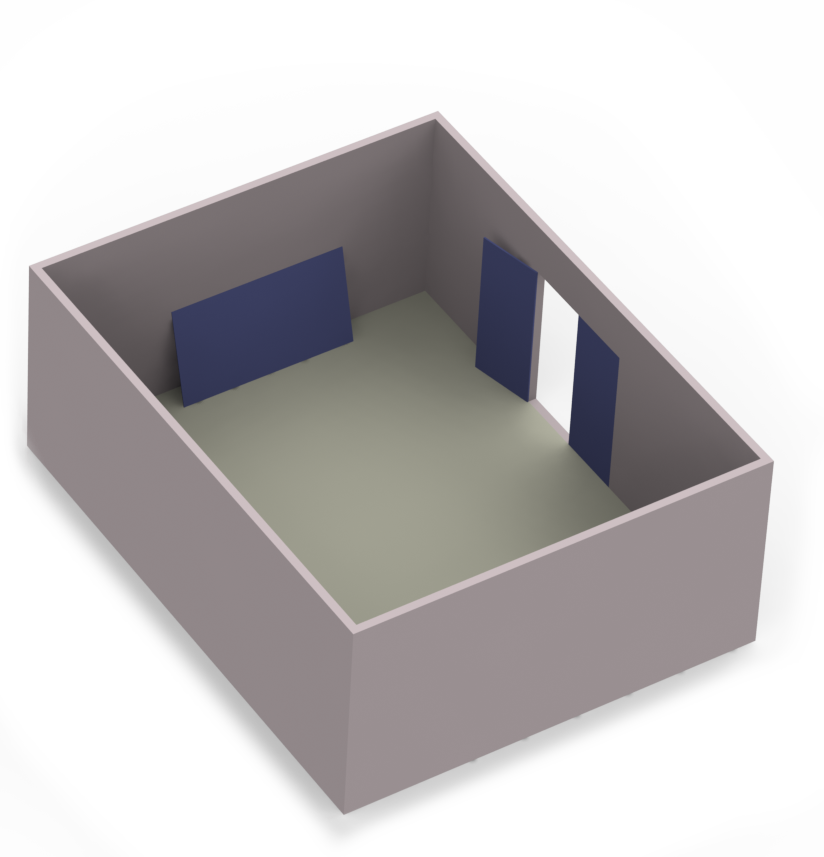
\includegraphics[scale=1.0]{033_cad_02}
		\caption{CAD Modell der Umgebung}
		\label{fig.mapMod}
	\end{center}
	%\vspace*{-8mm}
\end{figure}

Für den Einsatz des \kps{s} ohne vorhandene aktuelle Modelldaten kann eine Kartierung \red[(Mapping)] der Umgebung erfolgen. Die Kartierung von 2D- und 3D-\red[Umge-bungen] ist in aktuellen Forschungen eng mit der Lokalisation innerhalb dieser Umgebungen verknüpft.\red[ Begriff Karte hier einführen?] Ein verbreitetes Forschungsfeld in diesem Zusammenhang ist das simultane Kartieren und Lokalisieren in unbekannten Umgebungen \red[(engl. \textit{Simultaneous Localization And Mapping}, kurz SLAM)]. Dabei existieren verschiedene Algorithmen und Implementierungen zur Lösung der Problemstellungen. Die Kartierung selbst soll in dieser Arbeit nicht näher erläutert werden, für eine detailliertere Darstellung sei deshalb auf \red[\cite{Durrant2006}] verwiesen.\\

Zur Validierung des Systems wurde die in \abb{fig.mapSLAM} dargestellte Umgebung aufgezeichnet. Dabei wurde eine Implementierung \cite{Rgbdslam} nach Endres \textit{et al.} \cite{Endres2014} verwendet, welche die SLAM Anwendung mittels einer RGB-D Kamera realisiert. Das \kps{} kann somit auch für die Kartierung der Umgebung eingesetzt werden.\\

\begin{figure}[ht]
	\begin{center}
		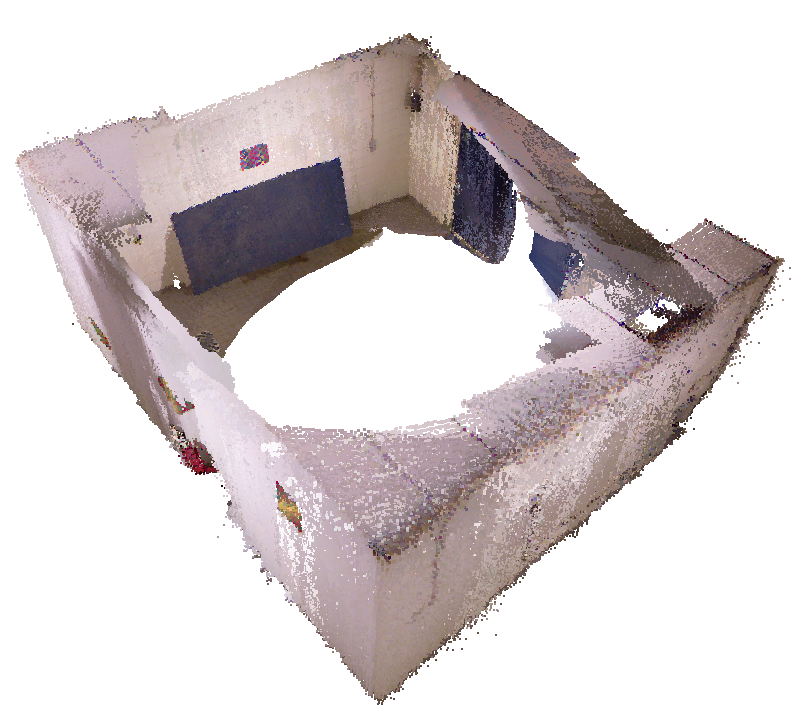
\includegraphics[scale=0.25]{pointcloud_meshlab}
		\caption{Karte RGBDSLAM Subfigures: echter raum (?) - Punktewolke}
		\label{fig.mapSLAM}
	\end{center}
	%\vspace*{-8mm}
\end{figure}

Das Ergebnis der Kartierung entspricht einer texturierten Punktwolke. Im Gegensatz zu der Ableitung aus vorhandenen Modelldaten handelt es sich daher nicht um geschlossene Geometrien. Da die Umgebung selbst jedoch ohnehin nicht als Teil der Projektion eingesetzt wird hat dies keine Auswirkungen auf die Funktionalität des Systems. Nachteiligen Einfluss können jedoch die im Vergleich zu Modelldaten geringere Auflösung sowie die Rauscheinflüsse des Kinect-Sensors zeigen. Die Güte eines Modells aus der Kartierung liegt meist unter der Modellgüte bei Ableitung aus vorhandenen 3D-Daten. Durch Verwendung der selben Sensoren während der Kartierung und der Lokalisation können die Fehlereinflüsse jedoch leicht verringert werden, da wiederkehrende Sensoreinflüsse so bei beiden Verfahren auftreten.\\

\section{Modellobjekte}
Für die Projektion der visuellen Zusatzinformationen sind zu Grunde liegende Modelldaten erforderlich. Modellobjekte beschreiben somit alle Strukturen und Objekte, welche keine Elemente der realen Umgebung abbilden. Die zur Erstellung der Modellumgebung eingesetzten Verfahren können ebenso auf die Modellierung von Objekten und Strukturen angewendet werden. Anstelle von Algortihmen zur Kartierung der Umgebung lassen sich dabei jedoch spezielle Verfahren zur Erfassung dreidimensionaler Objekte einsetzen, wie beispielsweise von Xu \textit{et al.} \cite{Xu2012} beschrieben.\\

Anders als die Modellumgebung müssen die Modellobjekte jedoch nicht als reale Objekte vorhanden sein, weshalb die Modellgüte auch keine Auswirkungen auf die Lokalisations- oder Projektionsgenauigkeit hat. Es können somit beliebige Objekte modelliert werden um diese später in der realen Umgebung zu visualisieren.  Für die Visualisierung ist jedoch eine ausreichende Auflösung der Modellstrukturen und -texturen anzustreben. \abb{fig.modobj} zeigt zwei Beispiele möglicher Modellobjekte und ihre Integration in die Modellumgebung.\\

\begin{figure}[ht]
	\begin{center}
	\subfigure[Modellobjekt Steckdose]{
		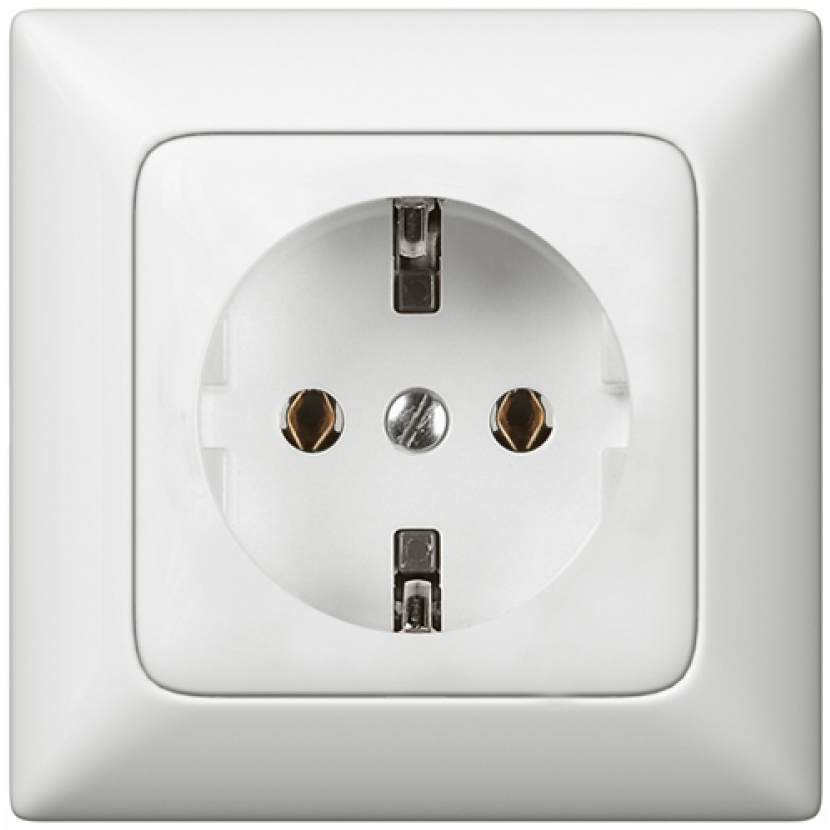
\includegraphics[scale=0.15]{steckdose}
	}
	\hspace{3mm}
%	\subfigure[Modellobjekt elektrische Leitung]{
%			
\includegraphics[scale=1.0]{spacer}
%	}
%	\hspace{3mm}
	\subfigure[Modellobjekte in Modellumgebung]{
		
\includegraphics[scale=1.0]{spacer}
	}
	\caption{Modellobjekte, Subfigures (insgesamt 4, jeweils allein und in Umgebung| Reichen 3? 2xModell + zusammen in Umgebung?): Steckdosen - Leitungen}
	\label{fig.modobj}
	\end{center}
	%\vspace*{-8mm}
\end{figure}

\section{Dateistruktur}
Um die Szene, bestehend aus der Modellumgebung und allen integrierten Modellobjekten, später wieder in den virtuellen Planungsablauf integrieren zu können wird eine Dateistruktur definiert, welche die Sicherung der aktuellen Modellkonfiguration ermöglicht. Alle Modellelement werden dazu mit ihrer aktuellen Pose, Textur und geometrischen Repräsentation erfasst und aufgezeichnet. Eine Wiederherstellung verschiedener Konfigurationen ist damit ebenfalls jederzeit möglich.\\
\red[Dateiformat? YAML? Eine Datei enthält alle Informationen über die Welt und über die einfügbaren Objekte (Preview Funktion). Hinzufügen/entfernen von Objekten zur Datei möglich, suchen nach vorhandenen Objekten in Datenbank möglich?]